\documentclass[aspectratio=169]{beamer}
\usepackage{graphicx}
\usepackage{hyperref}
\usetheme{metropolis}
\title{Gantt Charts}
\institute{Engineers for Exploration, UC San Diego}
\logo{
\includegraphics[height=.65cm,keepaspectratio]{e4e_logo_350x136.png}}
\setbeamertemplate{caption}[numbered]
\begin{document}
\maketitle
\begin{frame}
    \centering
    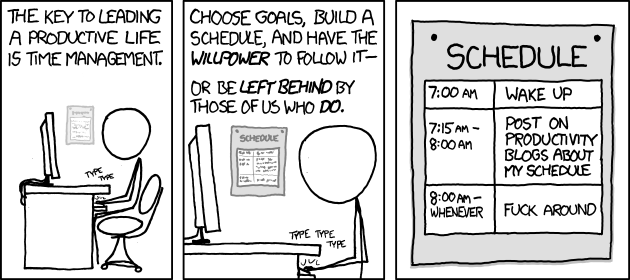
\includegraphics[width=0.8\textwidth]{xkcd_874_time_management.png}\footnote{\url{https://xkcd.com/874}}
\end{frame}
\begin{frame}
    How do we approach planning what needs to be done?
\end{frame}
\begin{frame}{Project Planning Example}
    Goal: Build a 10 ft x 10 ft shed to house a dog.

    Hint: We only have the dog right now...
\end{frame}
\begin{frame}
    \centering
    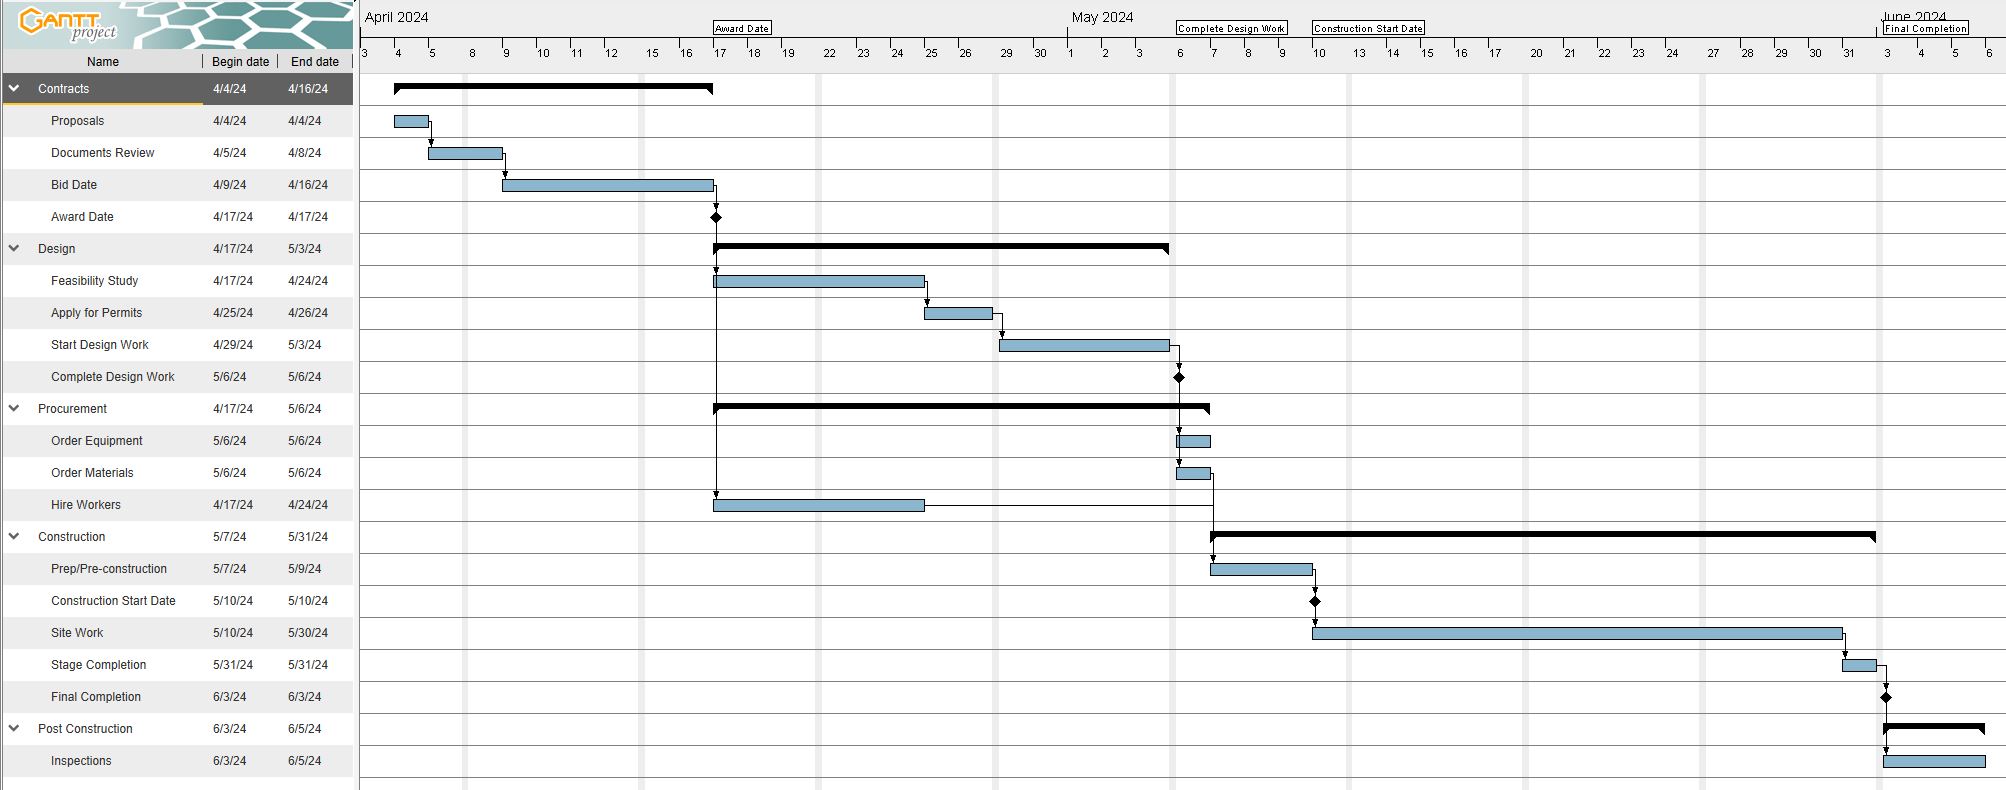
\includegraphics[width=\textwidth]{Construction-Gantt-chart-showing-task-lists-and-due-dates.png}
\end{frame}
\begin{frame}{What are the advantages of Gantt Charts?}
    \begin{itemize}
        \item Task Dependency
        \item Visualization of the Future
        \item Current Progression
        \item Availability of Slack
    \end{itemize}
\end{frame}
\begin{frame}{Gantt Chart Tools}
    \begin{itemize}
        \item GanttProject: \url{https://www.ganttproject.biz/download/free}
        \item Microsoft Project: \url{https://www.microsoft.com/en-us/microsoft-365/project/project-management-software}
        \begin{itemize}
            \item Or via \url{https://azureforeducation.microsoft.com/}
        \end{itemize}
    \end{itemize}
\end{frame}
\begin{frame}{MS Project}
    \centering
    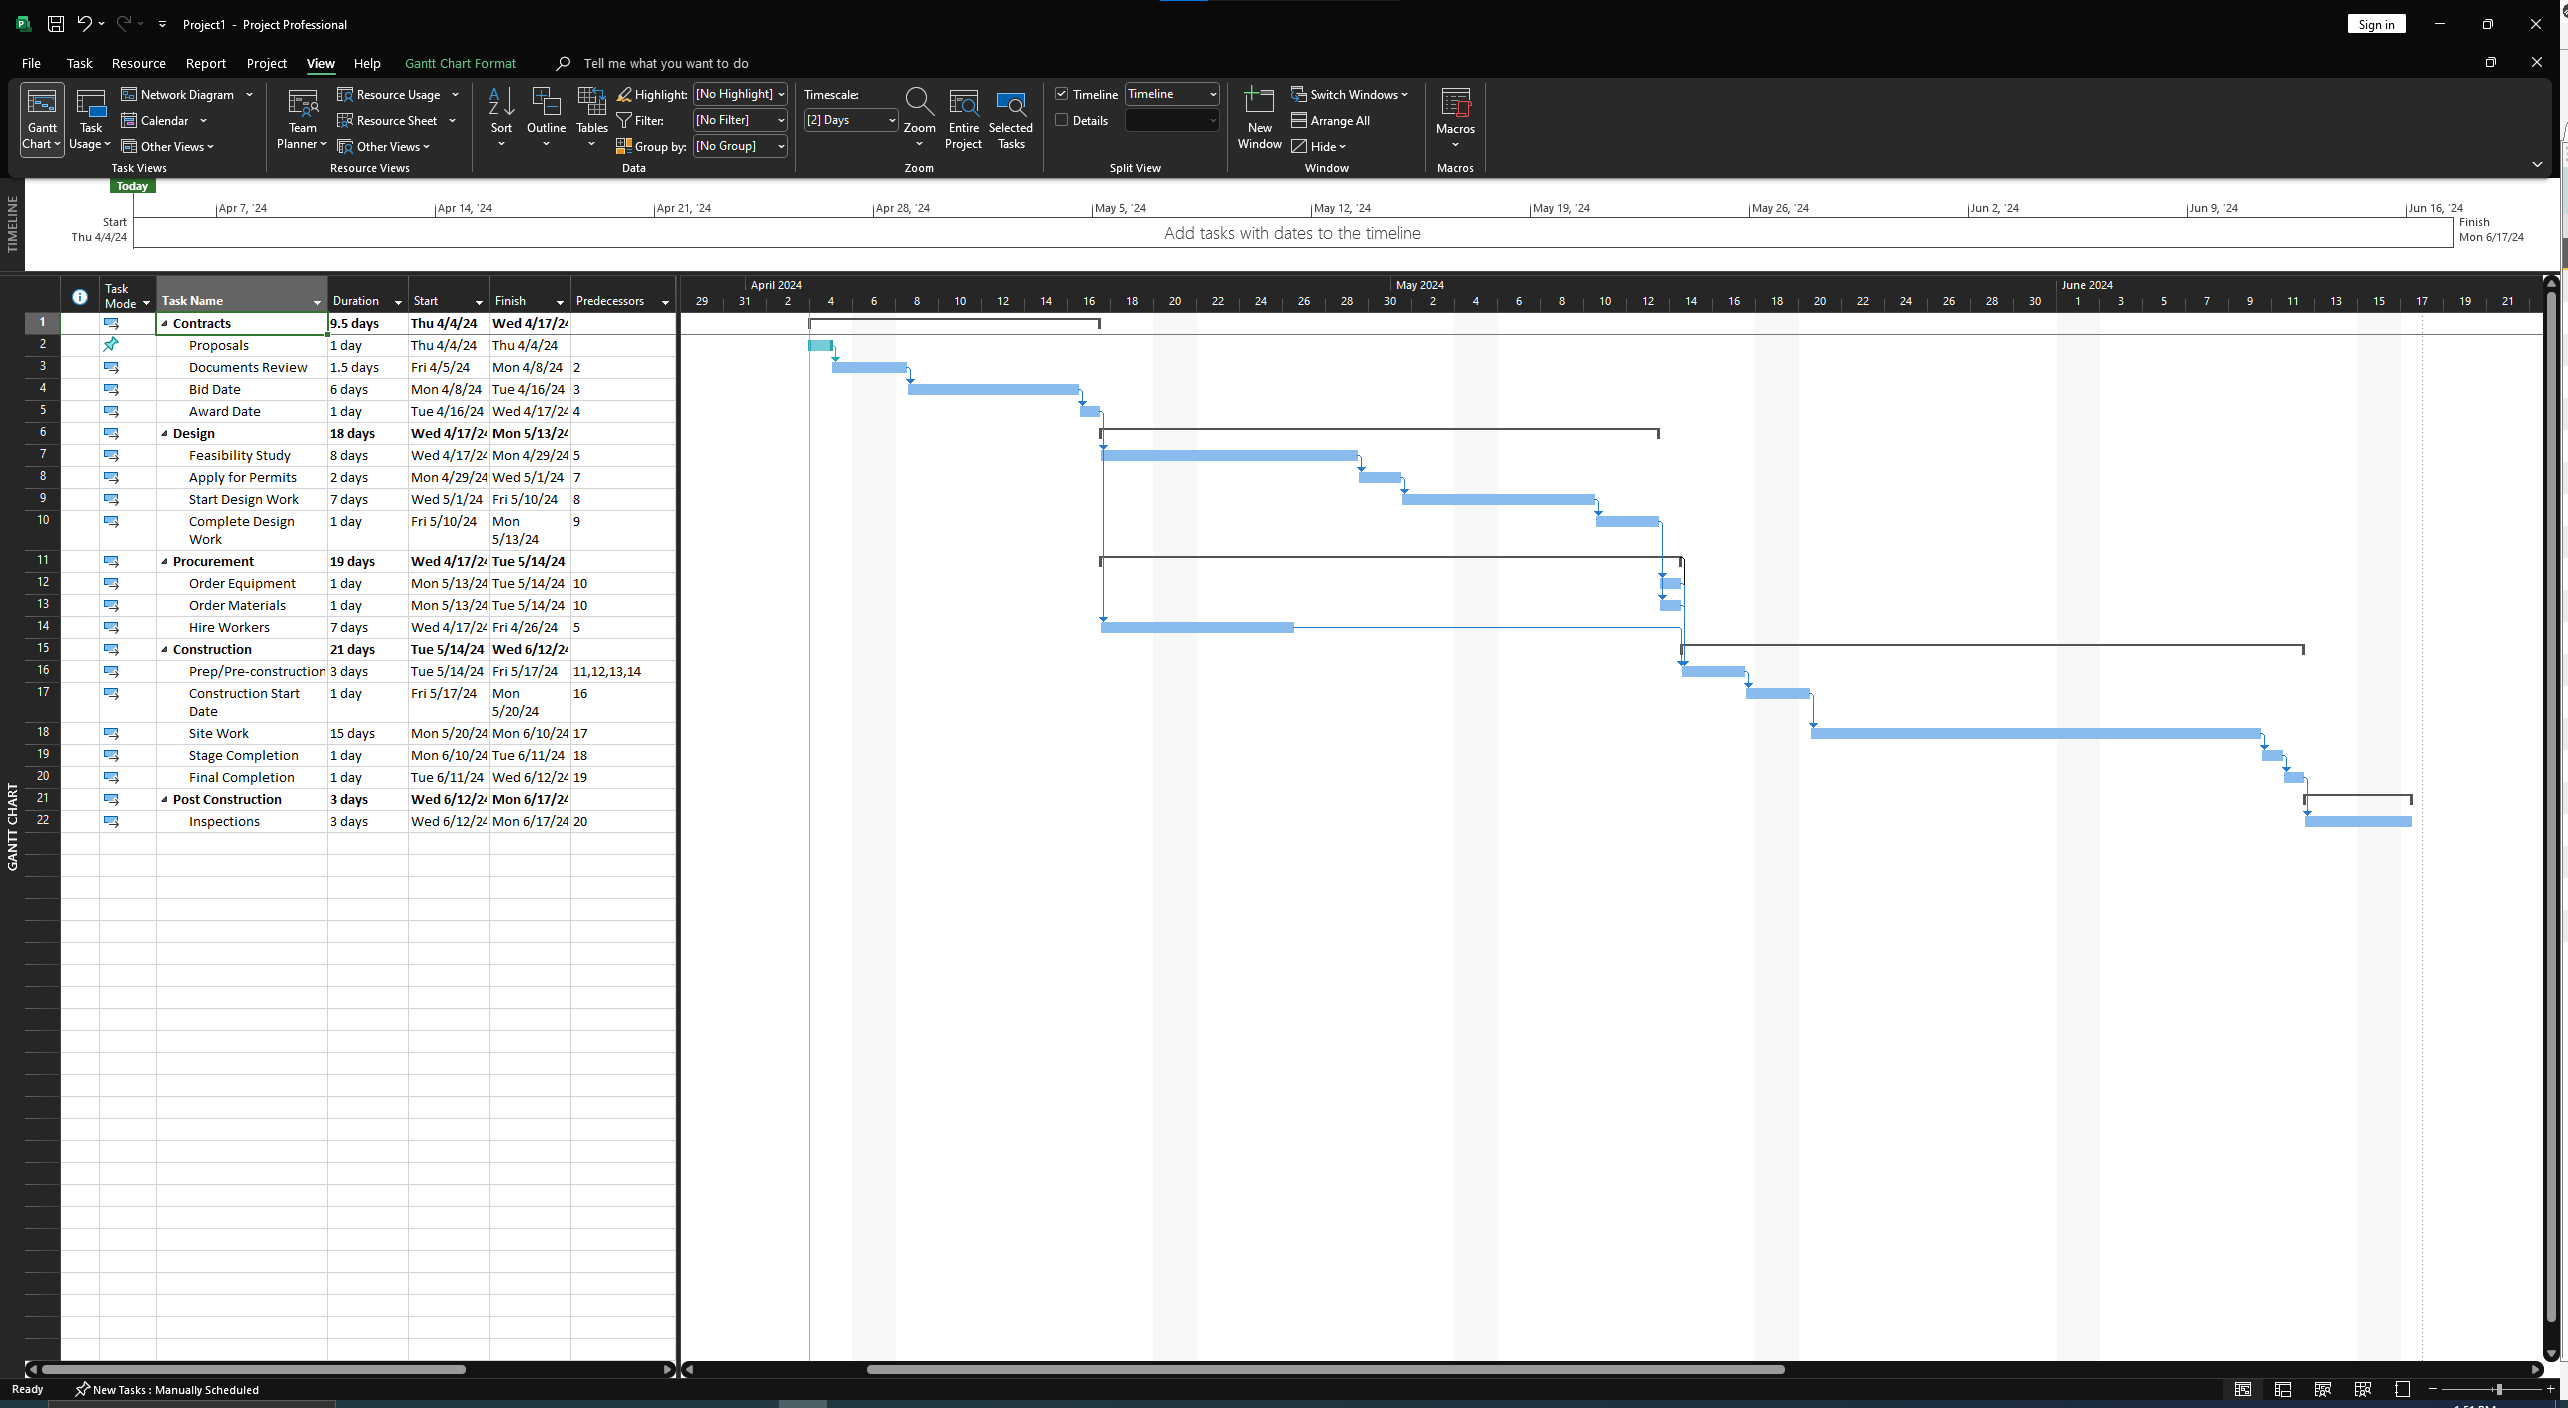
\includegraphics[width=0.8\textwidth]{14_ms_project.png}
\end{frame}
\begin{frame}{GanttProject}
    \centering
    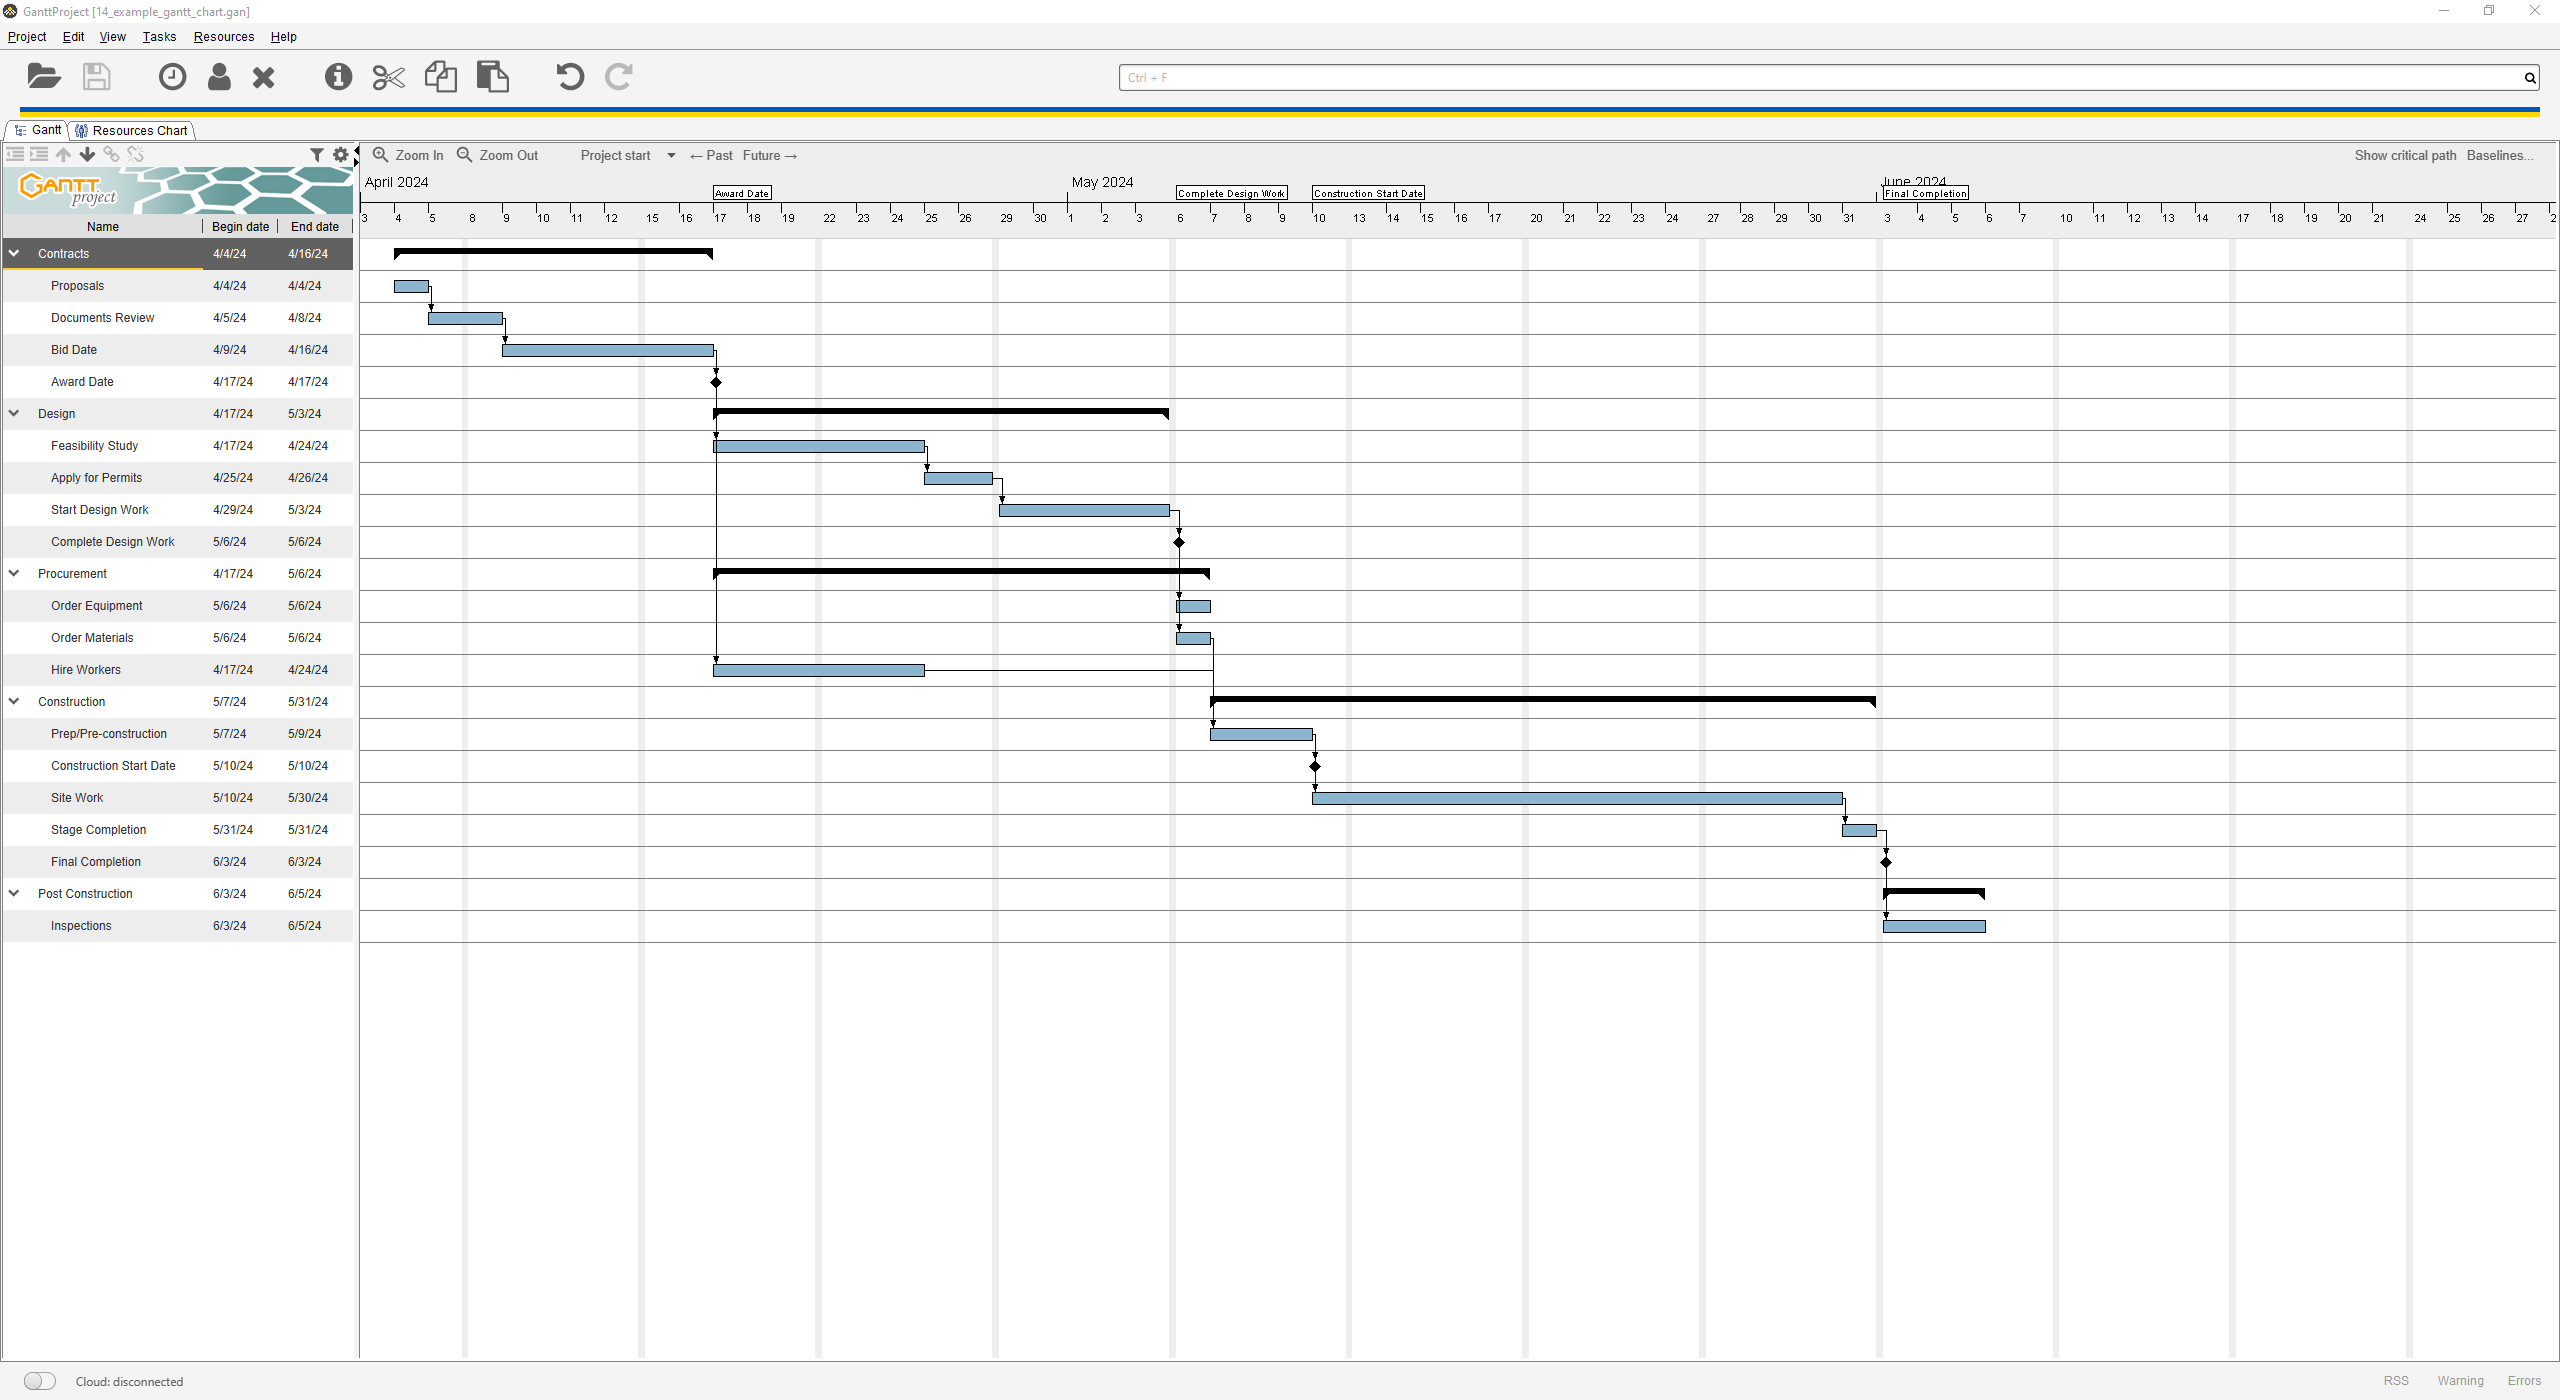
\includegraphics[width=0.8\textwidth]{14_ganttproject.png}
\end{frame}
\begin{frame}
    GanttProject Demo
\end{frame}
\begin{frame}{Project Planning Exercise}
    Goal: Build the FTC 2023-2024 blue pusher robot to compete in 4 months

    \url{https://youtu.be/6e-5Uo1dRic?si=9ZBnOwG9Bq8o19ql}
\end{frame}
\end{document}
